%%%%%%%%%%%%%%%%%%%
%% プリアンサンブル
\documentclass[10pt,a4j]{jarticle}
\usepackage{amsmath}
\usepackage[dvipdfmx]{graphicx}
\usepackage{subfigure}
\usepackage{here}
\usepackage[small, bf]{caption}

%maketitleの再設定
\usepackage[top=15truemm,bottom=15truemm,left=15truemm,right=15truemm]{geometry}
\makeatletter
 \renewcommand{\@maketitle}{\newpage
  %\null%%
  %\vskip 5.0em
 \begin{center}
   {\vspace*{0.1mm} \LARGE \@title \par} \vskip 1.5em 
   %{\normalsize \lineskip .5em \begin{tabular}[t]{l}\@author \end{tabular}\par}
   \vskip 1em {\large \@date} 
   \end{center}%%%
 \begin{flushright}%%%
  {\normalsize \lineskip .5em \begin{tabular}[t]{l}\@author \end{tabular}\par}
  \end{flushright}
 %\end{center}%%%\end{center}
 \par
 \vskip 1.5em}
 \makeatother

%thebibliographyの再設定
\makeatletter
  \renewenvironment{thebibliography}[1]{%
    \global\let\presectionname\relax
    \global\let\postsectionname\relax
    \subsection*{\refname}\@mkboth{\refname}{\refname}%%%%<-section
    \list{\@biblabel{\@arabic\c@enumiv}}%
          {\settowidth\labelwidth{\@biblabel{#1}}%
          \leftmargin\labelwidth
          \advance\leftmargin\labelsep
          \setlength\baselineskip{10pt}% 文字サイズ
          \setlength\itemsep{0zh}% アイテム間のマージン
          \@openbib@code
          \usecounter{enumiv}%
          \let\p@enumiv\@empty
          \renewcommand\theenumiv{\@arabic\c@enumiv}}%
    \sloppy
    \clubpenalty4000
    \@clubpenalty\clubpenalty
    \widowpenalty4000%
    \sfcode`\.\@m}
    {\def\@noitemerr
      {\@latex@warning{Empty `thebibliography' environment}}%
    \endlist}
\makeatother

%二段組の設定
\usepackage[]{multicol}
\setlength{\columnsep}{10truemm}

%章番号の終わりをドットで繋げる
\usepackage{secdot}
\sectiondot{subsection}
%bold vectorの定義
\newcommand{\bvec}[1]{\mbox{\boldmath $#1$}}
%ページ番号の消去
\pagestyle{empty} % すべてのページ番号を消去


%%%%%%%%%%%%%%%%%%
%% 文書設定 
\title{トピックモデルを用いたサッカーの攻撃パターンの分類による\\類似プレーの抽出}
\author{神谷 啓太(東京大学大学院 工学系研究科 社会基盤学専攻)\\
中西 航(東京工業大学 環境・社会理工学院 土木・環境工学系)\\
泉 裕一朗(東京大学大学院 工学系研究科 社会基盤学専攻)\\
〒113-8656 東京都文京区本郷7-3-1 TEL:03-5841-6118\\
E-mail:kamiya@trip.t.u-tokyo.ac.jp\\}
\date{\empty}


%%%%%%%%%%%%%%%%%%%
%% 原稿開始 
\begin{document}
%タイトル表示
\maketitle
\thispagestyle{empty} % 1ページ目を表示させない
%2段組本文の開始
\begin{multicols}{2}
%はじめに
\section{はじめに}
\label{sec:hajimeni}
数多くのスポーツで、センサやデータ計測員を駆使して多量のデータを取得し、統計的手法によってそれらを分析し、得られた示唆や知見をチーム戦略や選手評価に活用することが一般的となっている。
サッカーにおいても、ボール支配率やパス・シュート本数などの従来のスタッツを始め、ここ数年では選手の走った経路を逐次記録したトラッキングデータなどが計測されている。
サッカーでは両チーム合わせ22人の選手とボールが互いに影響し合いながら45分ハーフを連続的にプレーしており、取得されるデータにはそのような複雑な動きがすべて記録されている。
サッカーの試合の大局を俯瞰的に把握するためには、この複雑なデータから選手や観戦者にとって解釈可能な形で示唆や知見を発掘する研究や分析が望まれる。

関連する研究の一つとして、Kijimaら\cite{kij}はサッカーの試合展開を支配する単純な法則性に言及している。
一見複雑に見える選手とボールの位置変化はフラクタル構造を持つというもので、サッカーの試合はある普遍的な法則に従うことを示唆している。

しかし一方で、観戦者や選手が感じる「戦況」は試合中に大きく変化することがある。
例えば、攻勢であったのにいつの間にか守勢に転じている、停滞していた状況が一気に動き出す、などである。
このような戦況変化は上記の不変性の崩れとも考えられ、戦況変化を適切に把握することができれば、試合を有利に進めることに繋がる。
しかし現状、実際に試合を観戦もしくはプレーすること以外に戦況変化を把握する方法が存在しない。
戦況変化を自動的に抽出できれば試合を有利に進めるための戦略が立てられるだけでなく、観戦者に対する情報提供などの面で有用であり、その研究意義は大きい。

戦況変化の自動抽出に向け、まずは戦況変化とは何かを検討する必要があるが、上述した例はいずれも選手やボールの時系列的な振る舞いが変化した結果であると解釈できる。
そのため、選手やボールに関するデータの時系列的振る舞いをモニタリングし、その振る舞いが変化した点を検出することで戦況の変化を抽出することが可能となると考えられる。
以上を踏まえると、統計的変化点検出\cite{yam_dm}の枠組みを使用し、データの時系列的な振る舞いの変化点を検出することでサッカーの試合における戦況変化の抽出を行うことができると考えられる。

なお、サッカーを始めとする集団競技の戦況は、選手個々の意思決定に依る動きだけでなく、チーム全体としての動き、もしくは選手相互間やボールとの関係から発生するものである。
したがって戦況が代表されるようなある一つの変数を見つけることは難しく、複数の変数および変数間の関係に着目して分析する必要がある。
また、実用を考える上で、リアルタイムに戦況変化が抽出されることが望ましい。
すると、多次元時系列データを対象に、確率モデルとして時系列モデルを仮定して、リアルタイムに変化点度合いのスコアを計算していく手法であるChangeFinder\cite{yam_cf}が適用可能であると考えられる。

本研究の目的は、トラッキングデータを用いてサッカーの試合における戦況変化の抽出を行うことである。
第\ref{sec:cf}章でChangeFinderについて説明した後、第\ref{sec:input}章で分析に用いる変数を選定する。第\ref{sec:exp}章で実データにChangeFinderを適用し、検出された戦況変化に関する解釈を行う。最後に、本研究のまとめと今後の課題を第\ref{sec:owarini}章でまとめる。


%Latent Dirichlet Allocation
\section{トピックモデルを用いた類似プレーの抽出手法}
\label{sec:lda}
本章ではトピックモデルを用いた類似プレーの抽出手法について説明する。
まず、提案手法を構築するにあたり必要となるトピックモデル、LDA(Latent Dirichlet Allocation)について概説した後、サッカーにおける一連の攻撃をいかにトピックモデル的な観点から解釈可能かを議論する。
その後、トピックモデルを用いたサッカーのプレー内容の分類およびそれに基づく類似プレーの抽出手法について説明する。
なお、LDAについての解説は参考文献\cite{lda}\cite{topic_blue}\cite{topic_white}をもとに記す。

\subsection{Latent Dirichlet Allocation}
LDAは、もともと文書の確率的生成モデルとして提案されたモデルである。
ただし、文章の順序は無視し、Bag of Words(BoW)表現と呼ばれる単語と出現頻度のペアの集合をモデル化する。
ここで、BoW表現は単語が共起している現象を表しており、文書集合として考えると統計的に共起しやすい単語の集合がいくつか存在するはずである。
LDAは、この単語の共起性を統計モデルとして数理的に扱うために提案された。


\subsubsection{LDAの生成過程}
LDAでは、文書中の単語がどの潜在トピックによって生成されたかを示す潜在変数を導入する。
具体的には、文書$d$の$i$番目の単語を$w_{d,i}$として、対応する潜在変数を$z_{d,i}$と定義する。
潜在トピックの添字集合を$\{1,2,...,K\}$とする($z_{d,i}\in\{1,2,...,K\}$)。
各潜在変数の値は、それぞれ単語の出現分布$\phi_k(k=1,2,...,K)$に対応する。
つまり、文書中の各単語は離散値をとる潜在変数を背後に保持しており、その潜在変数の値が同じ単語はトピックに属する(同じ単語の出現分布に従う)というモデル化を行う。

文書数を$M$、文書$d$の文章長(総単語数)を$n_d$とする。
LDAでは、文章は複数のトピックから構成され、その構成比を離散分布としてもつ。
$\theta_{d,k}$を、文章$d$でトピック$k$が出現する確率(文章$d$でのトピック$k$の構成比率)とし、トピック分布を$\bvec{\theta}_d=(\theta_{d,1},\ldots,\theta_{d,K})$とする。
$\phi_{d,v}$をトピック$k$における単語$v$の出現確率とし、単語の出現分布を$\bvec{\phi}_k=(\phi_{k,1},\ldots,\phi_{k,V})$とする。
$\bvec{\theta}_d$や$\\bvec{phi}_k$は確率ベクトルであるので、確率ベクトル上の確率分布であるDirichlet分布(Dirと表記)による生成を仮定する。
すなわち、
\begin{equation}
	\bvec{\theta}_d \sim Dir(\bvec{\alpha}), d=1,\ldots,M
\end{equation}
\begin{equation}
	\bvec{\phi}_k \sim Dir(\bvec{\beta}), k=1,\ldots,K
\end{equation}

ここで、$\bvec{\alpha}=(\alpha_1,...,\alpha_K)$は$K$次元ベクトル、$\bvec{\beta}=(\beta_1,...,\beta_V)$は$V$次元ベクトルで、いずれもDirichlet分布のパラメータである。

単語$w_{d,i}$や潜在トピック$z_{d,i}$は離散値なので、多項分布(Multiと表記)を生成分布として仮定する。
すなわち、各文書$d(=1,...,M)$において、各単語は以下の生成過程を仮定する。
\begin{equation}
	z_{d,i} \sim Multi(\bvec{\theta}_d)
\end{equation}
\begin{equation}
	w_{d,i} \sim Multi(\phi_{z_{d,i}}) ,i=1,...,n_d
\end{equation}

%この生成過程のグラフィカルモデルを図\ref{fig:lda}に示す。



\subsection{トピックモデルとしてみるサッカーのプレー}
自然言語処理では、以下の仮定に基づいてトピックモデルを適用する。
\begin{itemize}
	\setlength{\itemsep}{0cm} % 項目間
	\item 文はいくつかのトピック(話題)の重み付き和で構成される
	\item トピックごとに使われやすい単語の分布がある
	\item 文は、トピック→単語の順で構成する単語数をサンプリングしたものである
	\item 文の中での単語の順番は不問とする、すなわち、順不同の単語から文の意味が一意に定まるとする
\end{itemize}

一方、本研究ではサッカーのプレーに対してトピックモデルを適用するにあたり、上記に対応するような以下の仮定を置く。
\begin{itemize}
	\setlength{\itemsep}{0cm} % 項目間
	\item 一連の攻撃は、ボール奪取時の状況やチームの特性に応じたトピック(攻撃パターン)の重み付き和で表現される
	\item 攻撃パターンごとに選択されやすいアクションや起こりやすい選手配置がある
	\item 一連の攻撃は、攻撃パターン→アクション/配置の順番に攻撃を構成する要素数をサンプリングしたものである
	\item 一連の攻撃内でのアクション/配置の順番は不問とする、すなわち、順不同のアクション/配置からプレー状況が定まるとする
\end{itemize}

最後の仮定について補足する。
直感的には、サッカーの一連のプレーにおいてプレーが生起する順番は意味を持ちそうである。
しかしながら、本研究では、仮に単語を適切に設定できれば、ある単語の集合を考えたときに起こりうるプレーの順番は実質的に定まると想定する。
このことにより、時系列データが格段に扱いやすくなるという大きなメリットがあるためである。
ただし、データから分析に有用な単語を生成する方法自体の検討が必要となるため、これを次章で説明する。
なお、この仮定には議論の余地が残るが、後述の適用において一定程度の妥当性は示されたと考えている。

\subsection{類似手法の抽出手法}
トピックモデルを用いて攻撃パターンを分類し、その分類結果に基づく類似プレーの抽出手法を以下の通り提案する。
\begin{enumerate}
	\setlength{\itemsep}{0cm} % 項目間
	\item ボールタッチ/トラッキングデータより文書を作成する
	\item 検索対象の文書$d_{req}$のトピック分布$\bvec{\theta}_{d_{req}}$を推定する
	\item データベース中の攻撃データ$d_{db}$とコサイン類似度$cos⁡(\bvec{\theta}_{d_{req}},\bvec{\theta}_{d_{db}})$ を計算
	\item その他検索条件(攻撃長、特定プレーの存在など)に基づき、類似度の高いものから抽出
\end{enumerate}





%入力変数の検討
\section{入力変数の検討}
\label{sec:input}

\subsection{使用したデータの説明}
本研究で使用したデータは、2016明治安田生命J1リーグ1stステージ第1節の計9試合に関して、
1/30秒毎にパスやタックルなどボール周辺で発生したイベントおよびその発生時刻と位置を取得したボールタッチデータと、1/25秒毎に選手及び審判のピッチ上での位置を取得したトラッキングデータの2種類である。
なお、これらのデータはデータスタジアム株式会社から提供を受けたものである。

\begin{figure*}[t]
  \begin{center} %センタリングする
    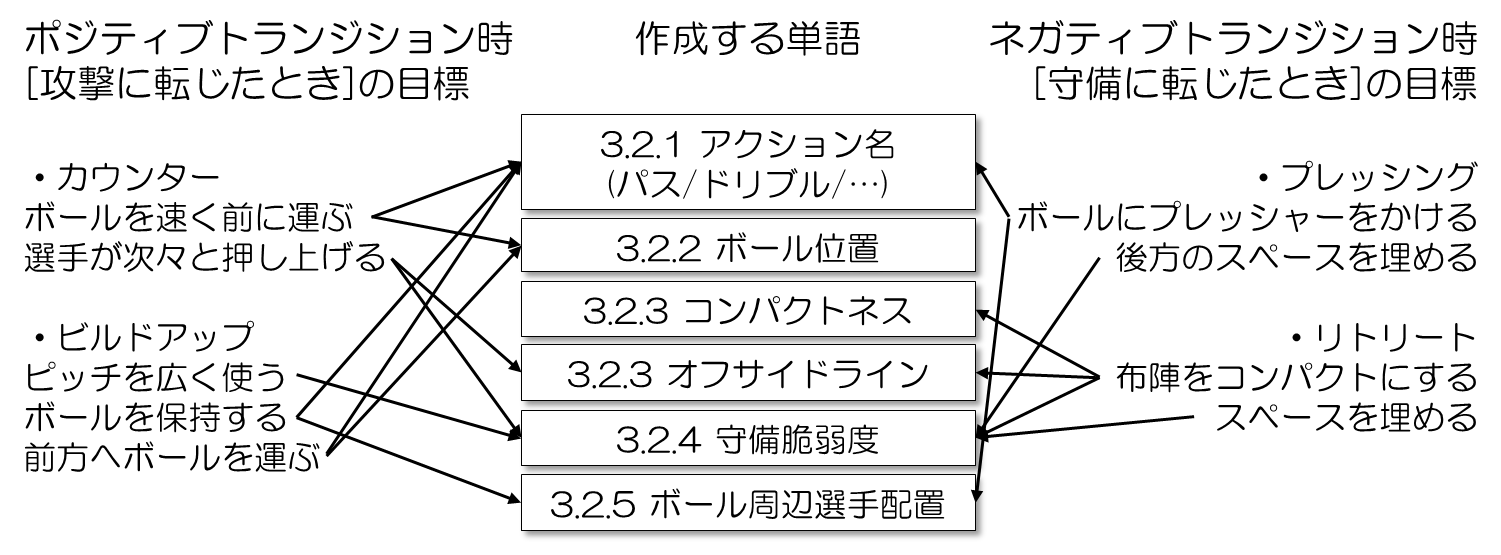
\includegraphics[width=12cm]{img/flow.png}
    %\renewcommand{\baselinestretch}{1}%
    \caption{サッカーの攻防の要素とそれを表す単語の作成}
    \label{fig:flow} %ラベルをつけ図の参照を可能にする
  \end{center}
\end{figure*}

\subsection{単語の作成}
LDAの適用のために、ボールタッチデータから本研究で用いる単語を作成する必要がある。
ここでの目標は、サッカーの一連の攻撃で発生している複雑な動きを、なるべく端的な単語の羅列で表現することである。そして、作成された単語を並べた文をみれば、人やボールの時系列の移動やその順序が表現される状態を目指す。
サッカーの一連の攻撃において実際に生起している事象をもとに検討し(図 \ref{fig:flow})、以下の5種類を作成することとした。



\begin{figure*}[htbp]
  \begin{center} %センタリングする
    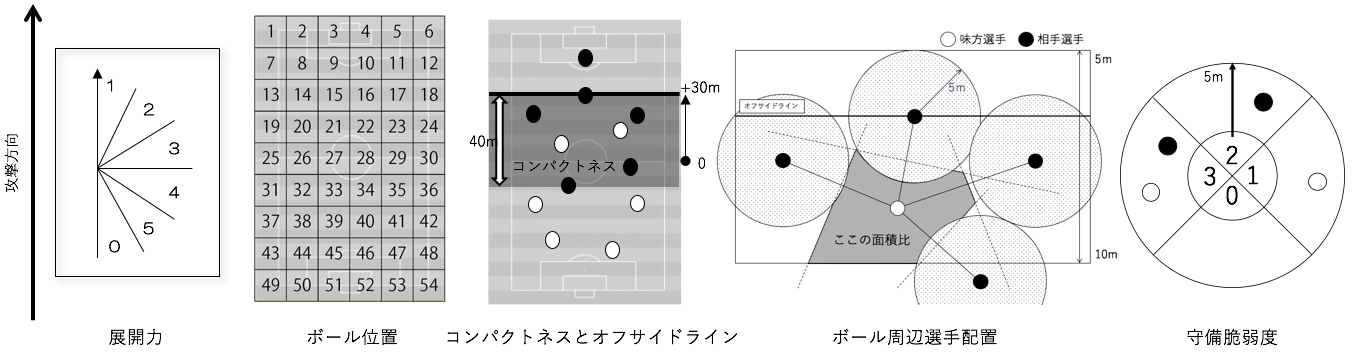
\includegraphics[width=18cm]{img/word.png}
    \renewcommand{\baselinestretch}{1}%
    \caption{作成した単語の例}
    \label{fig:word}
  \end{center}
\end{figure*}

\subsubsection{アクション名}
プレー内容を表現する単語として、ボールタッチデータに整理されている「アクション名」を選定した。
もともとはシュート、パス、GK、フィードなどの単語から構成されている。
ただし、「ホームパス」、「アウェイパス」および「トラップ」の出現回数が他の単語と比較してかなり多く、 特徴的な単語となりにくい可能性がある。
そこで、パスまたはトラップの向きとそのアクションが成功か否かを組み合わせたものをひとつの単語とする。
具体的には、提供されたデータ中の「展開力」と「成功F」を利用した。
例えば、
「パス」のアクションで、「展開力」が1方向、かつ成功の場合、生成される単語は「Pass\_1\_1」となる。
なお、一連の攻撃中に行われる守備側のアクションはすべて「defenseAction」という単語として統一した。


\subsubsection{ボール位置}
ピッチ上を54分割した上で、ボール位置を離散的に表現した単語を作成した。
これは、提供データ中の「hotzone6-9」と同義である。
図\ref{fig:word}にその定義を示す。


\subsubsection{コンパクトネスとオフサイドライン}
ピッチ上の選手配置として考えられる指標として、「コンパクトネス」および「オフサイドライン」を統合した単語を作成する。
コンパクトネスについて本研究では、「一番前方に存在する選手の$X$座標」と「後方より2番目に存在する選手の$X$座標」の距離をコンパクトネスと定義する。
各チームの選手がその時刻において、どれだけピッチ上で展開できているかを示す指標である。
また、オフサイドラインについては「後ろから2人目の選手位置」と定義し、ルール上のオフサイドラインとは異なる点に注意されたい。
この2つの指標は相関をもち、かつ選手がどれくらいの位置・幅でプレーをしているかを表すという点では重複した意味になる可能性がある。
そこで、「コンパクトネス×オフサイドライン」の組み合わせとして単語化することとする。
本研究では、10mずつ離散化して単語化かし、守備側の値のみを利用する。 

\subsubsection{守備脆弱度}
ピッチ上の選手配置のもうひとつの指標として、チームの守備力の脆弱性を表す単語を採用する。
ここでは自陣の最終ライン付近において相手選手が侵入している程度を守備脆弱度と定義する。
具体的には図\ref{fig:word}に示すように、「自軍のオフサイドラインより前方10m、後方5mの長方形のうち、最寄りの味方選手から5m以上離れており、最近傍選手が相手選手であるような地点の合計面積の割合」である。
こちらも守備側の配置のみを文章中の単語として利用する。

\subsubsection{ボール周辺選手配置}
ボール周辺に味方選手もしくは敵選手がいるかを表す単語として採用する。
ボールを中心に半径5mの円を想定し、4分割した各扇形セルそれぞれに、ボールに関与しているプレイヤーを除き、誰もいない場合は「0」、味方選手のみいる場合は「1」、敵選手のみいる場合は「2」、両方の選手がいる場合は「3」の文字を付加していく。
前・右・左・後の順に一つの単語を生成する。
図\ref{fig:word}に具体例を示す。
なお、(2016, 成塚ら)の分析により、「対戦相手との距離が5m以上近づくと、そこから次第に向きをそろえる傾向が強くなる」とされている\cite{2016nar}。
そこで、本研究でも近傍選手として考慮すべき距離を5mと設定した。







%適用結果
\section{戦況変化の抽出実験}
\label{sec:exp}

\subsection{適用条件}
ChangeFinderの入力変数として、ボール位置、前線位置、コンパクトネス(ホーム・アウェイチームごと)、守備脆弱度(ホーム・アウェイチームごと)、攻撃率の5種類・計7つのデータを7次元変数として設定した。
また、VARモデルの次数$K$は、オフラインでのVAR推定を行った場合の最小AIC値を参考に、$K=5$と決定した。
忘却率$r$や平滑化パラメータ$T,T′$についてはそれぞれ$r=0.01$、$T=50$、$T'=5$と設定した。
鹿島・湘南戦および松本・湘南戦の前後半のハーフ毎にChangeFinderを適用し、戦況変化の抽出を試みる。

なお、SDARアルゴリズムで用いるVARモデルの各種パラメータおよび統計量の初期値$\hat{\mu},\hat{\Sigma},C_i(i=1,...,K)$は、ハーフ開始60秒間で得られたデータから計算することとし、この間の変化点スコアは算出しない。

\subsection{適用結果および結果の考察}
松本・湘南戦後半を例として、図\ref{fig:res}の上段に入力時系列データ$\bvec{x}_t$を、下段にChangeFinderによる変化点スコアの出力値$Score(t)$を示す。
図\ref{fig:res}の上段において、1行目にボール位置と前線位置、2行目に湘南ベルマーレと松本山雅FCのコンパクトネス、3行目に湘南ベルマーレと松本山雅FCの守備脆弱度がそれぞれ灰色および黒色の実線で、そして4行目に松本山雅FCの攻撃率が示されている。
ボール位置と前線位置に関しては、正方向に値が上昇するにつれ、湘南ベルマーレの攻撃方向に進出していることを意味する。
下段は各時刻について算出された変化点スコア$Score(t)$であり、値が大きいほど戦況変化の度合いが大きいことを表している。

出力された変化点スコアを見ると、図中に(i)~(x)で示す合計10箇所で比較的大きな戦況変化が発生したと推定されたことが分かる。
紙面には掲載していないが鹿島・湘南戦前後半および松本・湘南戦前半の結果と比較すると、松本・湘南戦後半ではより高頻度で変化点が検出されていた。
松本・湘南戦後半では両チーム合わせ5つのゴールが生まれており、戦況の移り変わりが比較的大きかった試合であったことが、本結果において比較的高頻度に変化点が検出された理由として考えられる。

次に、検出された変化点が具体的にどういった戦況の変化を表しているのか、入力データの振る舞いと実際のプレーを比較することで結果の解釈および検証を行う。
ただし、図\ref{fig:res}からも分かるように入力データは複雑な動きをしているため、入力データから変化点検出の原因を直接分析するのは困難である。
そこで、パラメータ$\mu$の各時刻における推定値$\hat{\mu}$に着目する。
このパラメータはVARモデルの式(\ref{eq:var})より、自己回帰分を除いた平均的な値と解釈できる。
この推定値$\hat{\mu}$の振る舞いに着目し、検出された変化点との関係を分析することによって、どういった戦況の変化を表しているのか解釈を進めることが可能になると考える。

そこで、図\ref{fig:mu}に松本・湘南戦後半における推定値$\hat{\mu}$の推移と変化点の検出結果を示す。図中のグラフと変数の対応は図\ref{fig:res}と同様である。
図\ref{fig:res}で複雑な振る舞いをしていた入力値が、図\ref{fig:mu}の推定値$\hat{\mu}$では比較的滑らかな振る舞いをしていることが分かる。
また、推定値の時系列的振る舞いに変動があると、それ対応するように直後1分後あたりで変化点スコアが上昇していることが分かる。
なお、ChangeFinderでは第1段階および第2段階で移動平均処理を行っているため、観測データの入力から変化点の検出までに遅延が生じることに注意が必要である。

% 入力データと変化点スコアの出力
\begin{figure*}[htbp]
  \begin{center}
    \includegraphics[width=18cm]{img/res.eps}
    \renewcommand{\baselinestretch}{1}%
    \caption{松本・湘南戦後半における入力データおよび変化点スコア出力結果. 上段1行目にボール位置(ball)と前線位置(frontLine)、2行目に湘南ベルマーレと松本山雅FCのコンパクトネス(compact)、3行目に湘南ベルマーレと松本山雅FCの守備脆弱度(defence)をそれぞれ灰色および黒色で、4行目に松本山雅FCの攻撃率(attack)を示す。AWAYおよびHOMEはそれぞれ湘南ベルマーレと松本山雅FCに対応する。下段はChangeFinderによる変化点スコアの出力値$Score(t)$である。}
    \label{fig:res}
  \end{center}
\end{figure*}

%平均μと変化点スコアの出力および因果関係の考察
\begin{figure*}[htbp]
  \begin{center}
    \includegraphics[width=18cm]{img/mu.eps}
    \renewcommand{\baselinestretch}{1}%
    \caption{松本・湘南戦後半におけるパラメータ$\mu$の推定値$\hat{\mu}$の推移および変化点スコア出力結果. 図中のグラフと変数の対応は図\ref{fig:res}に同じ。なお、試合開始60秒間のパラメータは推定されていない。}
  \label{fig:mu}
  \end{center}
\end{figure*}

表\ref{tbl}に、各戦況変化点(i)~(x)について代表的な$\hat{\mu}$の変動の様子およびそれから想定される戦況変化の内容、ならびに実際にボールタッチデータから確認されたプレーの内容をまとめた。
例えば戦況変化点(i)の直前では、ボールが湘南攻撃方向に移動し、松本の守備脆弱度が上昇するという変動がパラメータ推定値$\hat{\mu}$の中で確認された。
この結果より、湘南が攻勢へと転換したことが戦況変化の内容として想定される。
実際にボールタッチデータより、湘南が複数のパスを繋ぎながら攻撃を展開している様子が確認できた。
他の変化点についても、表中にあるように、変化点スコア上昇の原因となるようなパラメータ推定値$\hat{\mu}$の変動から想定される戦況変化の内容が、実際のプレー内容と概ね合致していることが確認できた。

\begin{table*}[t]
  \centering
  \caption{検出された変化点の解釈および実際のプレーとの関係}
  \label{tbl}
  \begin{tabular}{|c|l|l|l|}
  \hline
  \# & 代表的な$\hat{\mu}$の変動 & 想定される戦況変化 & 実際に確認されたプレー  \\ \hline \hline
  i & \begin{tabular}[c]{@{}l@{}}ボールが湘南攻撃方向に移動\\ 松本の守備脆弱度が上昇\end{tabular} & 湘南の攻勢への転換 & 湘南がパスを繋ぎ攻撃を展開 \\ \hline
  i\hspace{-.1em}i & \begin{tabular}[c]{@{}l@{}}ボールが松本攻撃方向に移動\\ 湘南のコンパクトネスが低下\\ 松本のコンパクトネスが上昇\\ 湘南の守備脆弱度が上昇\\ 松本の守備脆弱度が低下\end{tabular} & 松本の攻勢への転換 & 松本がPKを獲得 \\ \hline
  i\hspace{-.1em}i\hspace{-.1em}i & \begin{tabular}[c]{@{}l@{}}湘南のコンパクトネスが上げ止まり\\ 松本のコンパクトネスが下げ止まり\\ 松本の守備脆弱度が回復\end{tabular} & 松本の守勢の実現 & 湘南がFKを獲得し松本が守備体勢に \\ \hline
  i\hspace{-.1em}v & \begin{tabular}[c]{@{}l@{}}ボールが松本攻撃方向に回復\\ 松本のコンパクトネスが上昇\end{tabular} & 松本の攻勢への転換 & 松本が自陣でFKを獲得しピンチを脱する \\ \hline
  v & \begin{tabular}[c]{@{}l@{}}松本のコンパクトネスが低下\\ 松本の守備脆弱度が上昇\\ 湘南の守備脆弱度が低下\end{tabular} & \begin{tabular}[c]{@{}l@{}}湘南の攻勢への転換\\ 松本の守勢の実現\end{tabular} & 湘南のCK/FKによる連続的な攻撃 \\ \hline
  v\hspace{-.1em}i & 湘南の守備脆弱度が回復 & 湘南の守備の実現 & 湘南得点後の松本キックオフ \\ \hline
  v\hspace{-.1em}i\hspace{-.1em}i  & 松本の守備脆弱度が低下 & 松本の守勢の実現 & 複数選手の交代により松本守勢の立て直しか \\ \hline
  v\hspace{-.1em}i\hspace{-.1em}i\hspace{-.1em}i & ボール位置が短時間に前後 & 試合の活性化 & 松本得点直後に湘南の得点 \\ \hline
  i\hspace{-.1em}x & \begin{tabular}[c]{@{}l@{}}ボールが松本攻撃方向に移動\\ 湘南の守備脆弱度が上昇\end{tabular} & 松本の攻勢への転換 & 松本のシュートを含む試合展開 \\ \hline
  x & \begin{tabular}[c]{@{}l@{}}ボールが松本攻撃方向に移動\\ 湘南の守備脆弱度が上昇\end{tabular} & 松本の攻勢への転換 & 同点弾を狙った松本の攻撃 \\ \hline
  \end{tabular}
\end{table*}

以上の結果を踏まえると、本分析方法により、攻勢・守勢への転換やセットプレーによる連続攻撃、連続得点による試合の活性化など、想定される戦況変化は概ね検出できていると考えられる。
ただし、実際の試合映像などを確認し、検出された戦況変化が妥当なものであるのか、また、未検出となった戦況変化等が存在しないかを専門的知見と共に検討を重ねたい。
また、現在は検出された変化点との関係をパラメータ$\mu$のみで見ているが、戦況のより高度な解釈に向け、$\mu$以外のパラメータについても精査を行う必要がある。
さらに、検出された戦況変化に対応するプレーにはセットプレーや選手交代などアウトオブプレーが多く含まれている。
実際、セットプレーを機に戦況が大きく変わることは多々あるが、変化点(i)や(x)などインプレー中の戦況変化の抽出も重要であろう。
インプレー中の戦況変化の抽出のためには、ChangeFinderに適用する時系列データからアウトオブプレー中のデータを排除する、一つのインプレーデータ毎にChangeFinderを適用するなど、分析方法を修正することが解決策として考えられる。




%おわりに
\section{おわりに}
\label{sec:owarini}

本研究では、統計的変化点検出手法であるChangeFinderをトラッキングデータに適用することで、サッカーの試合における戦況変化の抽出を行った。
ChangeFinderの入力変数の検討にあたっては、変数間の相関分析を通して共線性のない必要最低限な変数組となるよう配慮し、ボール位置、前線位置、コンパクトネス、守備脆弱度、攻撃率の5種類の指標を選定した。
松本山雅FC対湘南ベルマーレ戦後半のトラッキングデータにChangeFinderを適用した結果では、検出された合計約10か所の変化点に対応するように、その直前でパラメータ$\mu$の推定値$\hat{\mu}$の時系列的振る舞いに変動が確認された。
また、変化点スコア上昇の原因となるパラメータ推定値$\hat{\mu}$の変動から想定される戦況変化の内容と、実際のプレー内容がおおむね合致していることが確認できた。
本研究は、戦術変更が実戦況に効果を与えたか測定・分析するためのツールとして有用であると考えられる。

今度の課題として、実際の試合動画を専門的知見をもとに観察し、検出された戦況変化が妥当かつ十分なものであるか検証を進めたい。
また、より高度な戦術分析の実現に向け、VARモデルの$\mu$以外のパラメータについても精査し、変化点が検出された原因について分析を重ねる必要がある。
検出された変化点の前後でどのような戦況であったのか記述を行うことも今後の課題として挙げられる。
そして、データの背後に潜む戦況に関する潜在構造を推定し、戦況を変化させる因子の検出が可能となれば、より高度な戦術分析の実現へ向け前進するであろう。




%謝辞
\subsection*{謝辞}
本研究で使用したデータはデータスタジアム株式会社様に提供いただきました。
また、本研究の貸与データは情報・システム研究機構の新領域融合研究プロジェクト『社会コミュニケーション』データ中心科学リサーチコモンズ事業『人間・社会データ』の支援を受けたものです。
ここに、感謝の意を表します。

%参考文献
\begin{thebibliography}{9}
\bibitem{foot}Football LAB(フットボールラボ)とは、Football LAB ~サッカーをデータで楽しむ~、http://www.football-lab.jp/pages/about/、2017年1月31日閲覧
\bibitem{lda} Blei, David M., Andrew Y. Ng, and Michael I. Jordan. "Latent dirichlet allocation." Journal of machine Learning research 3.Jan (2003): 993-1022.
\bibitem{topic_blue} 岩田具治:トピックモデル、講談社、2015.
\bibitem{topic_white} 奥村学:トピックモデルによる統計的潜在未解釈、コロナ者、2015.
\bibitem{2016nar} 成塚拓真、卯田純平、山崎義弘:サッカーの対戦的特徴に現れる普遍的な統計性の探求、統計数理研究所共同リポート363、スポーツデータ解析における理論と事例に関する研究集会、第3巻、pp. 83-90、2016.
\bibitem{dtm} Blei, David M., and John D. Lafferty. "Dynamic topic models." Proceedings of the 23rd international conference on Machine learning. ACM, 2006.
\bibitem{tot} Wang, Xuerui, and Andrew McCallum. "Topics over time: a non-Markov continuous-time model of topical trends." Proceedings of the 12th ACM SIGKDD international conference on Knowledge discovery and data mining. ACM, 2006.

\end{thebibliography}


\newpage
\end{multicols}
\end{document}
